\documentclass[a4wide]{report}

\usepackage{amsmath}
\usepackage[a4paper, total={7in, 10.2in}]{geometry}
\usepackage{graphicx}
\usepackage[portuguese]{babel}
\usepackage[utf8]{inputenc}


\begin{document}

\noindent
{\bf Rafael V. Cacilhas  - Relatório 09 (\today)}

\vspace{0.5cm}

\section*{Exercício 1}



Sabemos  que as componentes da força $\vec{F_{kj}}$ são dadas por:

$\begin{cases} 
Fx = |F_{kj}|\cos\theta \\ 
Fy = |F_{kj}|\sin\theta
\end{cases} $

.

\subsection*{c) }

Na Figura \ref{2b1} temos os resultados para a energia em função do tempo para os métodos de Rouge-Kutta, Verlet (original) e Velocity-Verlet, respectivamente. Nesta escala, apenas para o método Verlet original temos que a energia total não aparenta ser constante, devido aos erros do método. Este fato mostra que apesar do erro do método Velocity-Verlet não ser tão pequeno quanto o do método de Rouge-Kutta ele ainda se apresenta como uma aproximação melhor do que o método de Verlet original.

\begin{figure}[!htb]
\centering
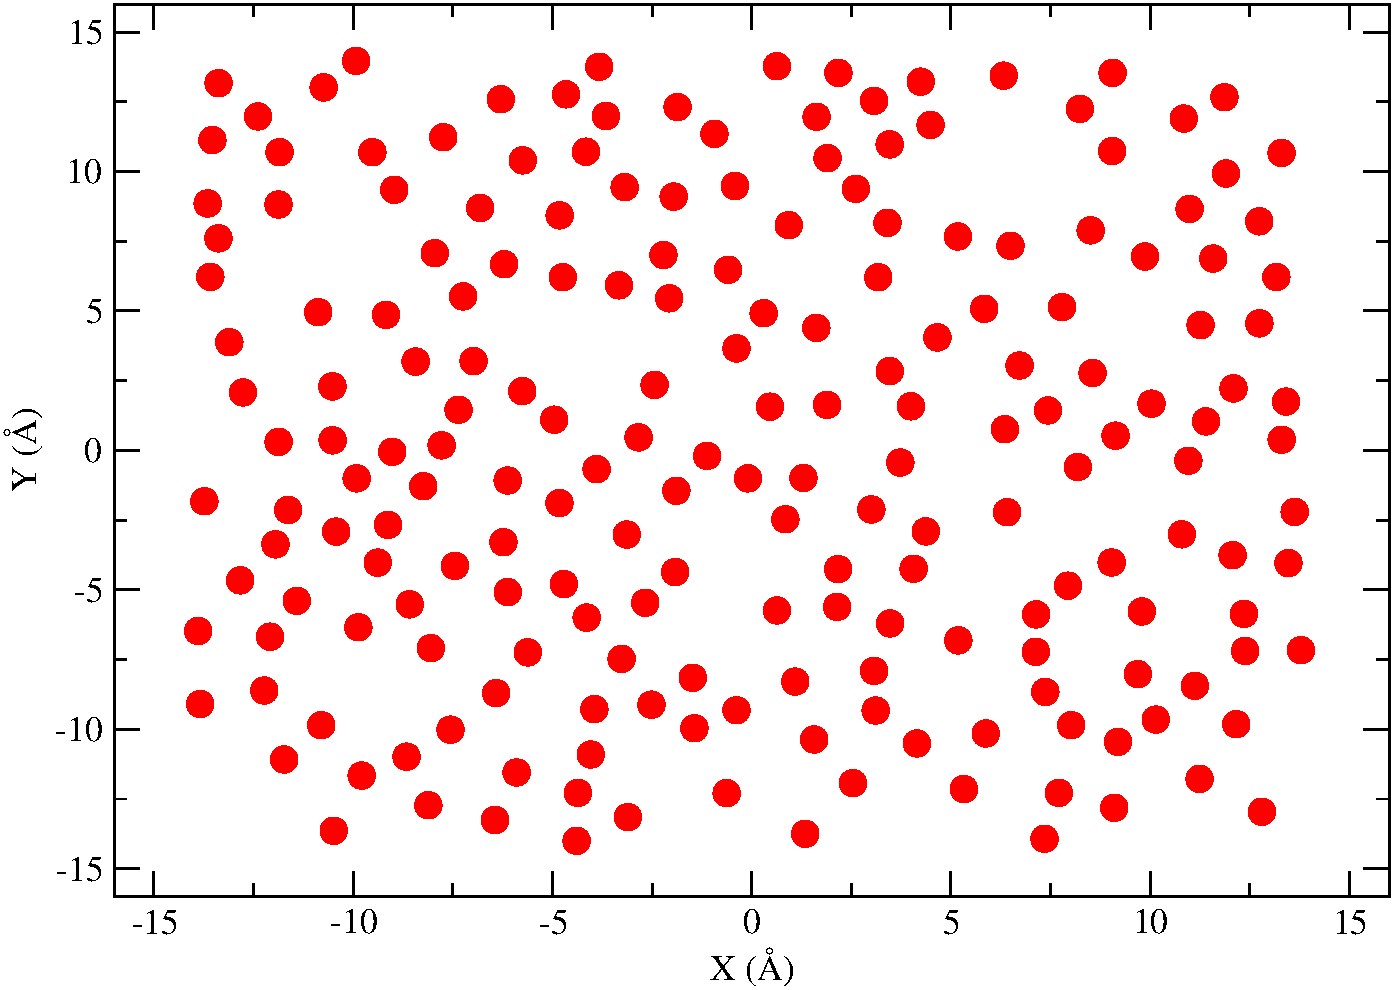
\includegraphics[width=0.4\textwidth]{mapa.pdf}
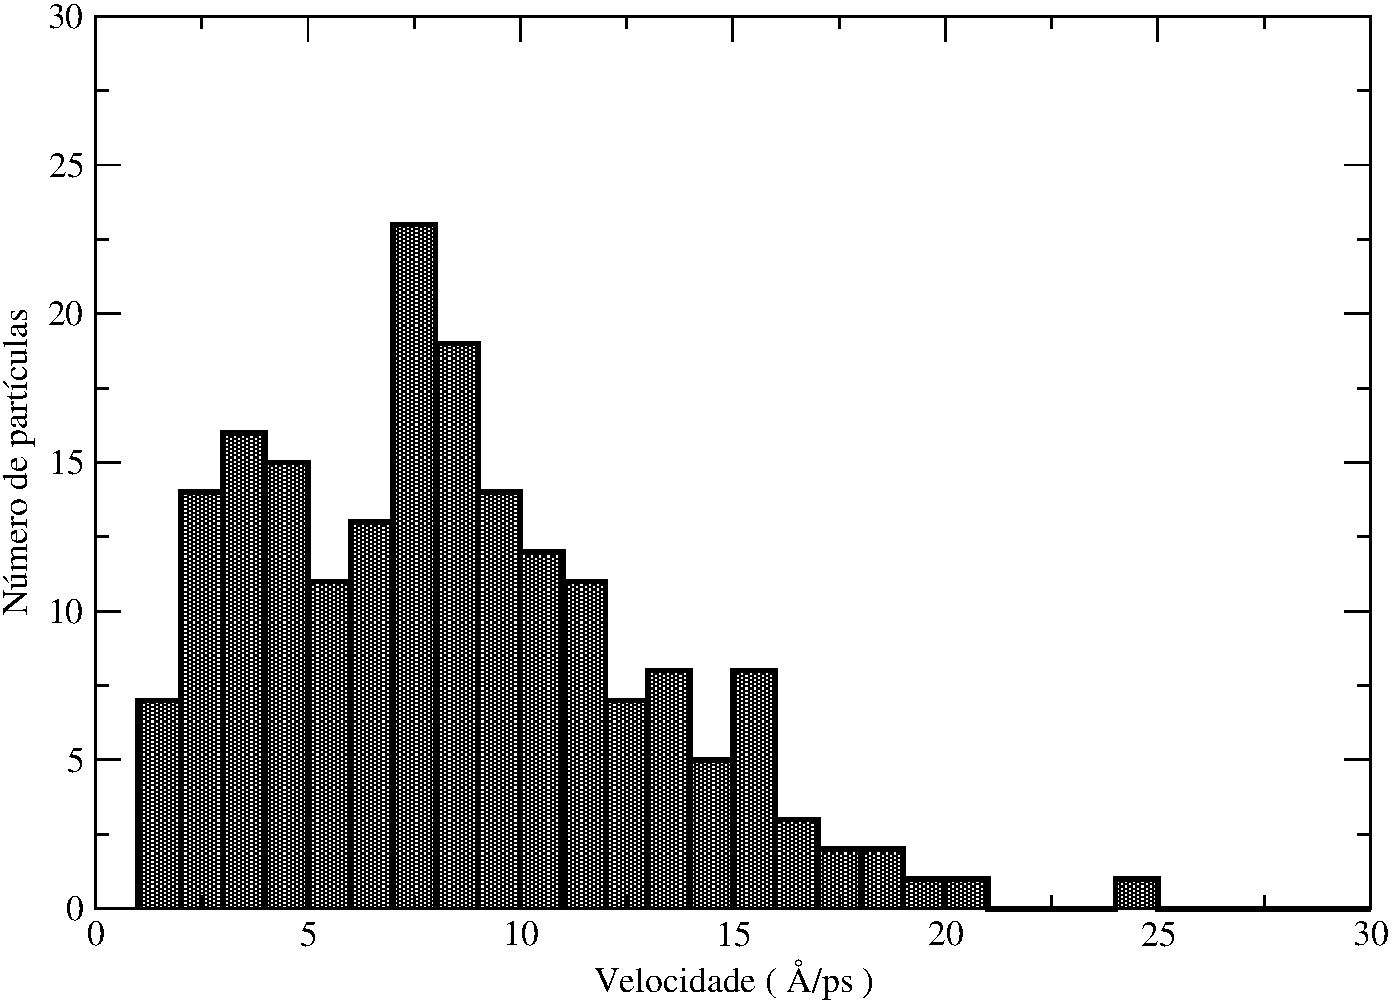
\includegraphics[width=0.4\textwidth]{hist.pdf}
\caption{Energias cinética, potencial e total para as condições iniciais 1.}
\label{2b1}
\end{figure}
\end{document}


\begin{figure}[!htb]
\centering

\caption{Energias cinética, potencial e total para as condições iniciais 1.}
\label{hist}
\end{figure}
\end{document}
